\documentclass[11pt, twoside]{report}
\usepackage[utf8]{inputenc}
\usepackage[english]{babel}
%\usepackage{times}
\usepackage{verbatim}
\usepackage[table,xcdraw]{xcolor}
\usepackage{titlesec}
\usepackage{epsfig}
\usepackage{subcaption}
\usepackage{gensymb}
\usepackage{wrapfig}
\usepackage{array}
\usepackage{tocloft}
\renewcommand{\cftsecaftersnum}{.}
\usepackage{secdot}
\usepackage[colorlinks=true, linkcolor = black]{hyperref}
%\usepackage[usenames, dvipsnames]{color}
\usepackage{fancyhdr} %header
\usepackage[Lenny]{fncychap}
\usepackage[a4paper, portrait, margin = 1.3in]{geometry}
\usepackage[utf8]{inputenc} %For
\usepackage[T1]{fontenc}
\usepackage{amssymb} %for R of real number
\usepackage{amsmath}% for "n times"
\usepackage{makeidx} %making index


\pagestyle{fancy}
\fancyhf{}
\fancyhead[LE]{\textbf{\thepage}}
\fancyhead[RE]{\textbf{\nouppercase{\leftmark}}}
\fancyhead[RO]{\textbf{\nouppercase{\rightmark}}}
\fancyhead[LO]{\textbf{\thepage}}

\fancypagestyle{plain}{%
  \renewcommand{\headrulewidth}{0pt}%
  \fancyhf{}%
}

\usepackage{etoolbox}
\makeatletter
%\ patchcmd{<cmd>}{<search>}{<replace>}{<success>}{<failure>}
\patchcmd{\chaptermark}{\@chapapp\ }{}{}{}
\makeatother

\newcommand{\red}[1]{\textcolor{red}{#1}}
\newcommand{\blue}[1]{\textcolor{blue}{\textbf{figure: #1}}}
\newcommand{\teal}[1]{\textcolor{teal}{\textbf{equation: #1}}}
\newcommand{\purple}[3]{\textcolor{purple}{\textbf{\textit{#1}, #2, #3}}}


\begin{document}

%%%%%%%%%%%%%%%%%%%%%%
%%%%%%%%%%TITLE PAGE%%%%%%%
%%%%%%%%%%%%%%%%%%%%%%%
\begin{titlepage}
    \begin{center}
        \begin{figure}[hbt!]
             \centering
             
\includegraphics[width=0.4 \textwidth]{./figures/unimi_logo_tesi}
        \end{figure}
        \textbf{\Large{UNIVERSIT\`A DEGLI STUDI DI MILANO}}\\
        \vspace{12pt}
        \Large{FACOLT\`A DI SCIENZE E TECNOLOGIE}\\
        \Large{DIPARTIMENTO DI FISICA}\\
        \Large{Corso di Laurea triennale in Fisica (L-30)}
        \vspace{24pt}
        \hrule
        \vspace{24pt}
        \textbf{\Large{Quantum Walks with Time-Dependent Hamiltonians}} \\ 
        
    \end{center}
    \vspace{120pt}
    \begin{flushleft}
        Relatore : 
        \textbf{Prof. Matteo G.A. Paris}\\
        Correlatore: 
        \textbf{Prof. Stefano Olivares}\\
        Correlatrice: 
        \textbf{Dott.sa Claudia Benedetti}
    \end{flushleft}
    \vspace{12pt}
    \begin{flushright}
        Candidato:\\
        \textbf{Matteo Garbellini}\\
        Matricola 885615\\
    \end{flushright}
    %\begin{flushright}
    %    Pacs: 98.65.-r
    %\end{flushright}
\end{titlepage}
\newpage

%%%%%%%%%%%%%%%%%%%%%%
%%%%%%%%%%ABSTRACT%%%%%%%
%%%%%%%%%%%%%%%%%%%%%%%
\newpage
\thispagestyle{empty}
\textbf{\Large{Abstract}} \\ \\
\noindent
In this thesis we study the properties of quantum walks with time dependent hamiltonian, focusing in particular on the application to the quantum search problem on graph. We compare the time independent and the time dependent approach for two graph topologies, the circular and the complete graph, which represent respectively the worst and best case scenario for the known quantum search. We also investigate the role of the function that regulates the time-dependance of the hamiltonian in the time scaling at which the solution is found. Lastly we exploit the consequences of the adiabatic theorem to study the localization properties of the time-dependent approach.

%%%%%%%%%%%%%%%%%%%%%%
%%%%%%%%%%TABLE OF CONTENTS%%%%%%%
%%%%%%%%%%%%%%%%%%%%%%%
\newpage
\thispagestyle{empty}
\tableofcontents

%%%%%%%%%%%%%%%%%%%%%%
%%%%%%%%%%PRELIMINARIES%%%%%%%
%%%%%%%%%%%%%%%%%%%%%%%
\newpage
\thispagestyle{empty}
\chapter{Preliminaries}

\section{Graph Theory}
A graph G is defined as a ordered pair $(V,E)$, where V is a set of vertices and E is a set of edges, which represent the connection between any two pair of vertices. If indeed any two vertices $(i,j)$ are connected by an edge we define as adjacent, and from this we can construct the \textit{adjacency matrix} A as:
\begin{equation}
A_{ij} = \begin{cases} 1 & (i,j)\in G \\ 0 & \mbox{otherwise} \end{cases}
\end{equation}
which represents the connectivity of the graph. We can then describe the degree of each vertex of the graph, namely the number of vertices (excluding itself) connected to it, through the \textit{degree diagonal matrix} $D_{jj} = deg(j)$.\\
It is also useful to introduce the \textit{laplacian matrix} defined as
\begin{equation}
  L = A-D
\end{equation}
which we'll later see describes the quantum walk evolution.\\
In the quantum realm a vertex is a vector in an N dimensional Hilber space, so that a vertex $|j\rangle$ can be represented in the following way
\begin{equation}
  |j\rangle = \begin{pmatrix} 1 \\ 0 \\ 0 \\ .. \\0 \end{pmatrix}
\end{equation}

Throughout this work we focus our attention on two particular graph topologies: the \textbf{circular} graph and the \textbf{complete} graph (FIG. 1).


\begin{figure}[ht]
\centering
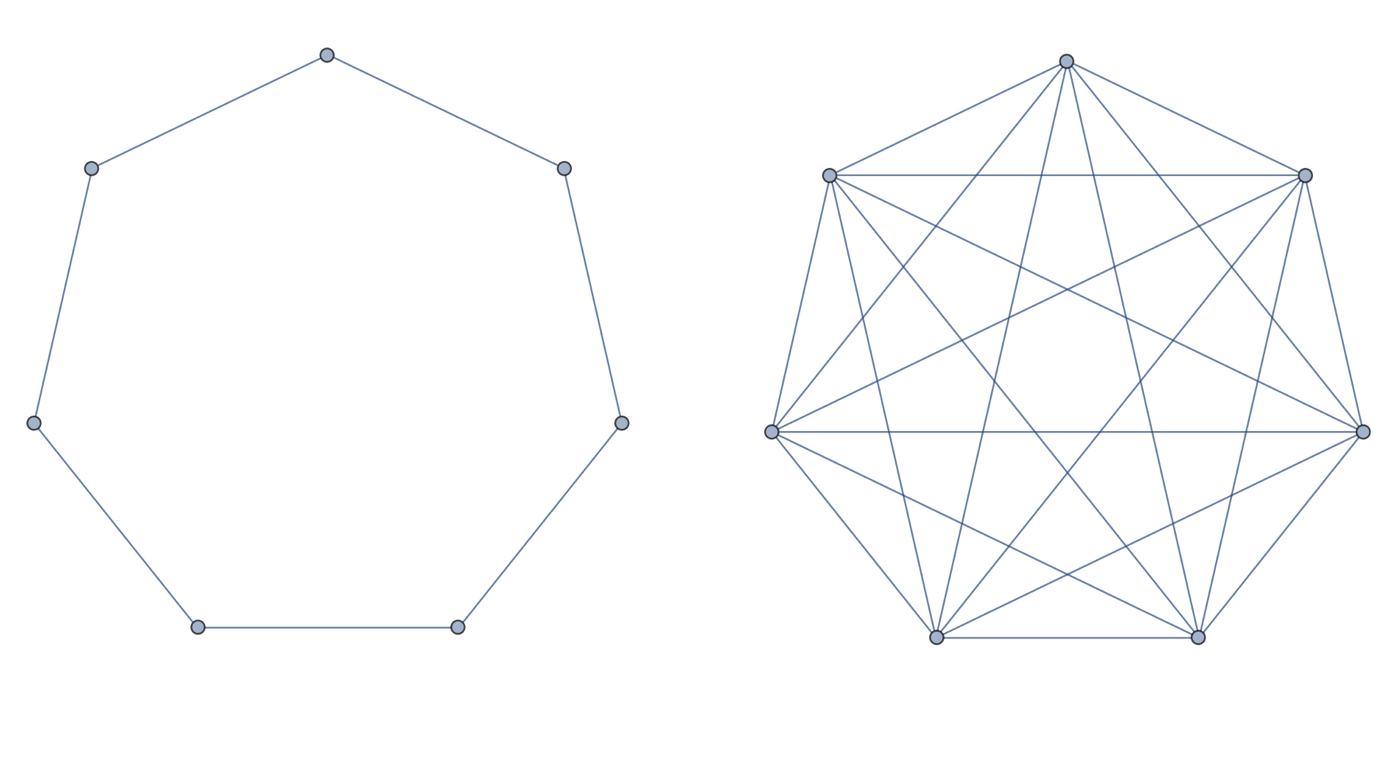
\includegraphics[width=9.5cm]{./figures/graph.png}%
\caption{Pictorial representation of a circular graph (left) and a complete graph (right) with N=7}
\end{figure}

\section{Quantum Walks}
The continous time quantum walk is the direct analougue of the classical random walk. Given a graph G, a random walk is a Markov process with a fixed probability for unit time $\gamma$ of jumping to an adjacent vertex $j$. This particular walk can be described by a linear differential equation in terms of probability, namely

\begin{equation}
  \frac{d}{dt}p_j(t) = \gamma\sum_{k}L_{jk}p_k(t)
\end{equation}

where $p_j(t)$ is the probability of being on the vertex $j$ at time $t$.\\
The quantum analogue takes place in an N-dimentional Hilbert space spanned by the states (vertex) $|j\rangle$ of the graph G. Instead of considering the classical probability as we previosuly did, we consider the probability time-dependent amplitudes $q_j(t) = \langle j|\psi(t)\rangle$, where $|\psi\rangle$ is a general time-dependent state. The differential equation takes thus the form of

\begin{equation}
  i\frac{d}{dt}q_j(t) = \sum_{k}H_{jk}q_k(t)
\end{equation}
The continous-time quantum walk is defined by letting $H=-\gamma L$, where $L$ is the previosuly defined Laplacian matrix.

\section{Grover's Quantum Search}
\red{This section should include the standard Grover's Quantum Search to give the contex for the quantum walk approach.}

\section{Quantum Search with Continous-Time Quantum Walk}
\purple{Spatial Search by Quantum Walk}{A. Childs, J. Goldstone}{quant-ph/0306054v2}\\
We now address the quantum search problem firstly formulated as Grover's algorithm and then extending it to the search on a graph using quantum walks. \\
To approach the Grover problem with quantum walk it's necessary to modify the hamiltonian such that the vertex $|w\rangle$, i.e. the target, is somewhat special. Following Grover's oracle an oracle hamiltonian $H_w$ is introduced

\begin{equation}
  H_w = -|w\rangle\langle w|
\end{equation}

which in particular has energy zero for all but the vertex $|w\rangle$ for which it has enenergy $-1$. Therefore the Grover problem, i.e. quantum search, becomes finding the ground state of such hamiltonian. To do so we consider the time-independent hamiltonian of the form
\begin{equation}
  H = -\gamma L + H_w = -\gamma L -|w\rangle\langle w|
\end{equation}
where L is the laplacian of the graph, which contains the information of the dynamics over that particular graph topology. The evolution of the quantum walk is therefore governed by this hamiltonian.\\

The quantum search routine works as follow:
\begin{itemize}
  \item we consider the superposition of all possible states, namely
  \begin{equation}
    |s\rangle = \frac{1}{\sqrt{N}}\sum_j|j\rangle
  \end{equation}

  \item we find the evolved state using the hamiltonian for a time T $H$
  \begin{equation}
  |\psi(T)\rangle = U(T)|s\rangle  = \mbox{exp}\Big\{-\frac{i}{\hbar}HT\big\}|s\rangle
  \end{equation}
  (Note that this evolution is valid only for time-independent hamiltonians.)

  \item we then measure the state onto the target $|w\rangle$ and find the corrisponding probability
  \begin{equation}
    p = |\langle w|\psi(T)\rangle|^2
  \end{equation}

\end{itemize}

The objective is to find the optimal value of $\gamma$ so that the probability of the system of finding itself in $|w\rangle$ is as close as possible to 1 for the smallest T.

\section{Search on Complete Graph}
We now look at the search on a complete graph. This case is particularly interesting since it can be solved analitically\\
\red{to be continued}

\section{Adiabatic Theorem}
\purple{Quantum Computation by Adiabatic Evolution}{E. Farhi, J. Goldstone, S. Gutmann, M. Sipser}{quant-ph/0001106}\\


A quantum system evolves according to the Schroedinger equation
\begin{equation}
    i\frac{d}{dt}|\psi(t)\rangle = H(t)|\psi(t)\rangle
\end{equation}
and defining the instantaneous eigenstates and eigenvalues of H(t) by
\begin{equation}
    H(t)|l;t\rangle = E_l(t)|l;t\rangle
\end{equation}
such that $E_0(t) \geq E_1(t) \geq ... \geq E_{N-1}(t)$. \\
The adiabatic theorem states that if the gap between the two lowest energy levels, $E_{1}(t) - E_{0}(t) > 0$, is stritcly greater than zero then for $T\rightarrow \infty$ the probability of being in the ground state is equal to one, namely
\begin{equation}
    \lim_{T \to \infty} |\langle l=0;t = T | \psi(T)\rangle| = 1
\end{equation}
This means that if the system is chosen to evolve at a slow enough rate, the instantaneous hamiltonian will remain in the ground state throught the evolution. It is useful to consider a smooth one-parameter hamiltonian $H(s)$ such that $s=t/T$, with $t \in [0,T]$ so that $s \in [0,1]$.
Let's now define the energy minimum gap by
\begin{equation}
    g_{min} = \min_{0 \leq s \leq 1} (E_1(s)-E_0(s))
\end{equation}
In addition we can find a time lower bound $T^*$ such that for $T\gg T^{*}$ the probability is arbitrarily close to 1, in detail
\begin{equation}
    T \gg \frac{\varepsilon}{g^{2}_{min}}
\end{equation}
where
\begin{equation}
    \varepsilon = \max_{0 \leq s \leq 1} \Big| \Big\langle l=1;s\Big| \frac{dH(s)}{dt} \Big| l=0;s\Big\rangle\Big|
\end{equation}

Let's now discuss how to take advantage of the adiabatic theorem introducting the usual way in which the adiabatic evolution is implemented. It is often presented a problem hamiltonian $H_P$ whose ground state is not so straight forward to find; on the other hand we can prepare the system in abeginning hamiltonian $H_B$ whose ground state is known. The problem hamiltonian encodes the solution of the problem, while the beginning hamiltonian is a tool for easily preparing the state to be evolved. The adiabatic implementation then consists, assuming that the ground state of $H_P$ is unique, in having a time dependent hamiltonian $H(s)$ such that
\begin{equation}
    H(s) = (1-s)H_B + s H_P
\end{equation}
In this way we can prepare for $s=0$ the system in $H_B$ and let it evolve so that for $s=1$ it reaches $H_P$. Thanks to the adiabatic theorem, if it's made to evolve sufficiently slowly we will find ourself in the ground state of the problem hamiltonian, which is exactly the solution.



%%%%%%%%%%%%%%%%%%%%%%
%%%%%%%%%%METHODS AND RESULTS%%%%%%%
%%%%%%%%%%%%%%%%%%%%%%%
\newpage 
\thispagestyle{empty}
\chapter{Methods and Results}

Nella ricca bibliografia disponibile sul legame tra teoria ergodica e meccanica statistica è possibile rintracciare una serie di argomenti comuni, divenuti classici e ormai presenti nella maggior parte dei libri di testo. Seppure all'interno di questa linea non si sia raggiunto un consenso universale, secondo l'autore del presente lavoro è possibile identificare un numero minimo di \textit{sei ipotesi fondamentali} (logicamente indipendenti) caratteristiche di questo approccio. In questo capitolo, dopo una breve ricapitolazione delle nozioni fondamentali della teoria ergodica, si presenterà un'esposizione critica di queste ipotesi e si discuteranno i loro rapporti sistematici nella costituzione dello schema fondazionale. 

\section{Elementi di teoria ergodica}


%%%%%%%%%%%%%%%%%%%%%%
%%%%%%%%%%CONCLUSIONS%%%%%%%
%%%%%%%%%%%%%%%%%%%%%%%
\newpage
\chapter*{Conclusions}
\addcontentsline{toc}{chapter}{Conclusions}

%%%%%%%%%%%%%%%%%%%%%%
%%%%%%%%%%APPENDIX%%%%%%%
%%%%%%%%%%%%%%%%%%%%%%%
\newpage
\chapter*{Appendix}
\addcontentsline{toc}{chapter}{Appendix}

%%%%%%%%%%%%%%%%%%%%%%
%%%%%%%%%%BIBLIOGRAPHY%%%%%%%
%%%%%%%%%%%%%%%%%%%%%%%
\newpage
\chapter*{Bibliography}
\addcontentsline{toc}{chapter}{Bibliography}

\end{document}




